\section{Mapzen}
Mapzen Merupakan laboratorium pemetaan open source dibawah Samsung Accelatoryang membangun dan mendukung data dan software terbuka untuk mempromosikan ekosistem pemetaan yang sehat. Tim Pengembangan dari Mapzen merupakan salah satu divisi dari SRA (Samsung Research Amerika) yang berfokus pada komponen inti dari platform geo, termasuk pencarian, rendering, navigasi, dan data.

Aplikasi Mapzen memakai data dan software lisensi dari OpenStreetMap. Jadi apabila Anda memakai aplikasi Mapzen harus mempunyai account di OpenStreetMap. Aplikasi Mapzen dibangun berdasarkan project open source OpenScienceMap, Pelias, Open Source Routing Machine (OSRM, dan SDK open source dari Mapzen, dapat mengakses hardware GPS di perangkat mobile untuk fitur navigasi dan peta pada saat berjalan, mengendarai mobil maupun bersepeda.

Keunggulan dari produk Mapzen adalah penggunaan mesin rendering fleksibel yang disebut juga Tangram yang digunakan untuk menampilkan peta digital dalam nuansa 2D maupun 3D secara real-time. Mapzen dibangun dari berbagai peralatan open-source yang dikemas ke dalam layanan Web dan di hosting di server Mapzen.

\subsection{Tambahkan shapefile OSM2PGSQL ke QGIS}
Cara menambahkan shapfile OSM2PGSQL ke QGIS:
\begin{enumerate}
\item Jalankan QGIS dan tampilkan peta kosong.
\item Pada panel Browser, navigasikan ke folder dimana shapefile disimpan dan buka file 'bandung_indonesia.osm2pgsql-shapefiles'.
\item Perhatikan bahwa file tersebut berisi tiga shapefile, dinamai dengan tipe geometri: line, point ,dan polygon.
\item Klik dua kali pada layer line untuk membukanya di peta. contoh yang di klik adalah 'bandung_indonesia_osm_line'. \ref{micin1}
\begin{figure}[ht]
	\centerline{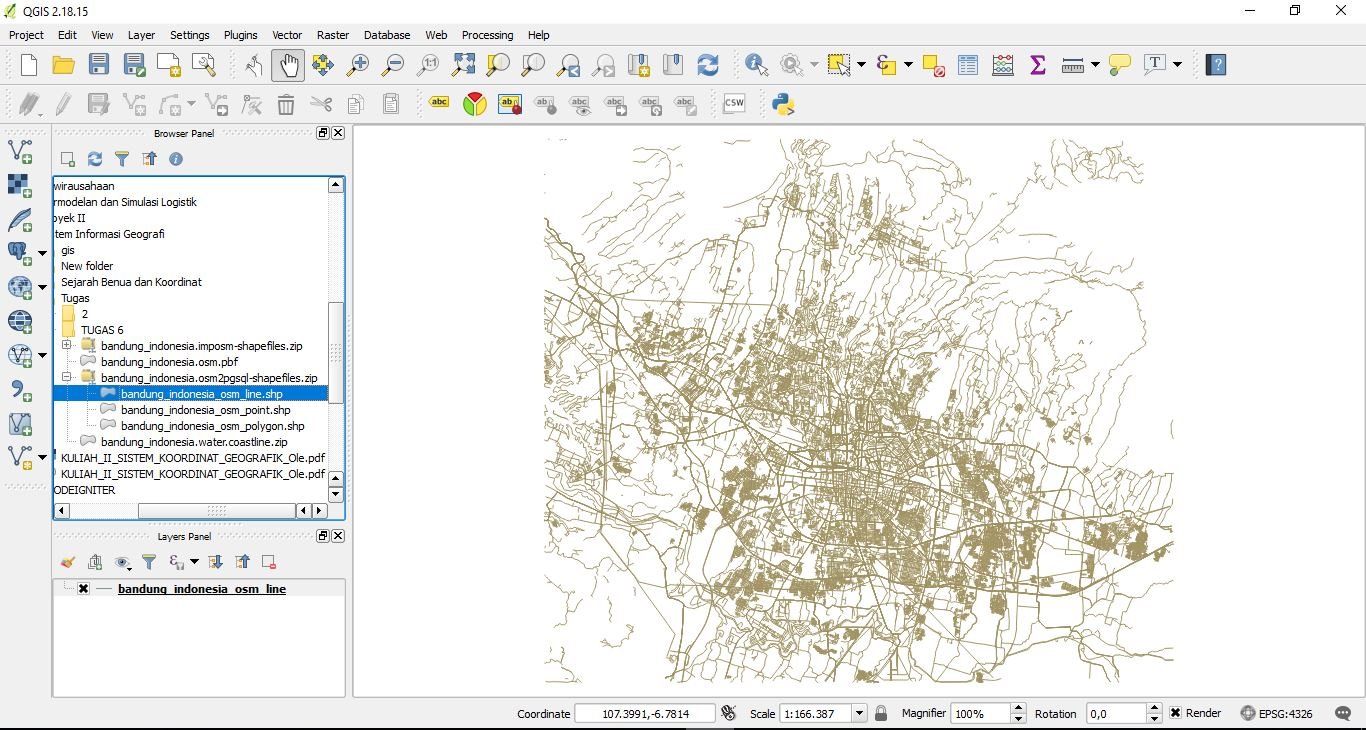
\includegraphics[width=1\textwidth]{figures/micin1.JPG}}
	\caption{OSM2PGSQL ke QGIS}
	\label{micn1}
	\end{figure}
